\appendix
\chapter{Anhang}

\begin{listing}[h]
\centering
\begin{minted}[linenos]{python}
#pseudocode
class Proc(object):
  def __init__(self, lookup):
    self.lookup = lookup or default_lookup()

  def run(self, step):
    proc = self.lookup[step.stepper](self, step)
    proc.run()
\end{minted}
\caption{Beispiel Zuordnung statt Fabrik}
\label{fig:fabrik-mapping}
\end{listing}


\begin{figure}
    \centering
    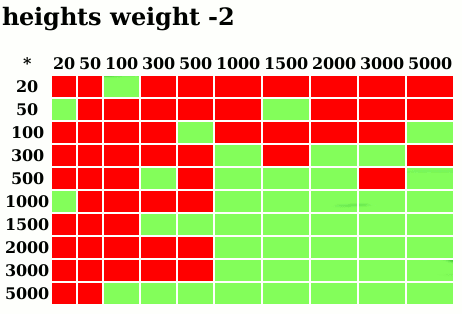
\includegraphics[width=4in]{images/exemplar-ausgabe.png}
    \caption{Bildschirmphoto Beispielerweiterung}
    \label{fig:beispielerweiterung-screenshoot}
\end{figure}

\begin{figure}
    \centering
    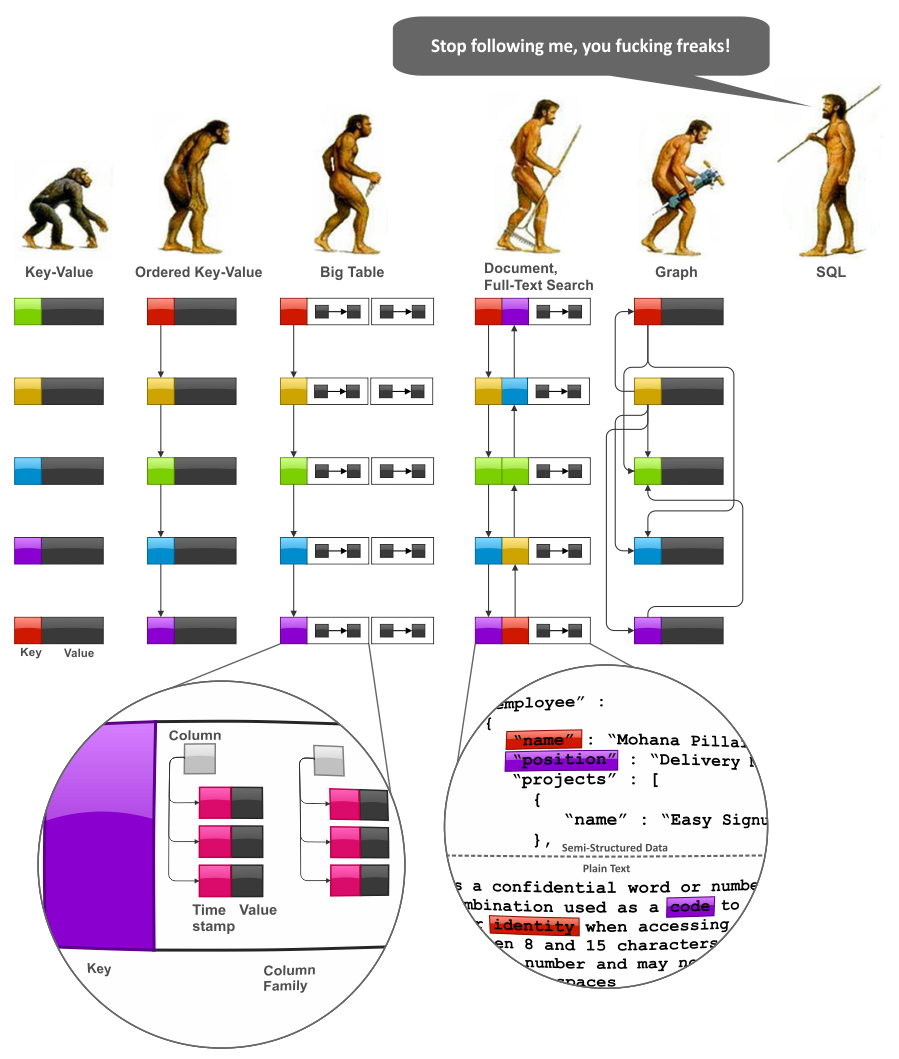
\includegraphics[width=\textwidth]{images/databases-overview.png}
    \caption{Übersicht Klassen an Datenbanken}
    \label{fig:klassen-datenbanken}
\end{figure}

\chapter{Anhang CD}

Im folgenden wird die Verzeichnissstruktur der CD grob umrandet:

\begin{itemize}
    \dhitem[Pfannschmidt\_CI.pdf] PDF-Version dieser Arbeit
    \dhitem[juggler] Das Projek wie in \cref{sec:imp:projektstruktur} beschrieben.
    \dhitem[evolve] Die Beispielerweiterung zur Datenanalyse.
    Sie ist im Detail wie folgt aufgebaut:
    \begin{itemize}
            \dhitem[funfind.py] Das Programm welches zum Generieren der Daten verwendet wird.
            \dhitem[composeapp] Die eigentliche Erweiterung als Spezifikation für CouchDB-compose.
            \dhitem[fill\_run.html] HTML-Datei mit den Ausgabedaten der Erweiterung aus dem Test ``Große Datenanalyse''
    \end{itemize}
\end{itemize}
